

\subsection{Disjoint Cycle Packing}
In this subsection we  design a PSAKS for the {\sc Disjoint Cycle Packing ()} problem. 
The parameterized optimization problem {\sc Disjoint Cycle Packing ()} is formally defined as,





We start by defining feedback vertex sets of a graph. Given a graph  and a vertex subset ,  is called a {\em feedback veretx set} of  if  is a forest. 
We will make use of the following well-known Erd\H{o}s-P\'{o}sa Theorem relating feedback vertex set and the number of vertex disjoint  cycles in a graph. 
\begin{lemma}[\cite{ErdosPosa1965}]
\label{lemma:erdosposa}
There exists a constant  such that for each positive integer , every (multi) graph either contains  vertex disjoint cycles or it has a feedback vertex set of size at most . Moreover, there is a polynomial time algorithm that takes a graph  and an integer  as input, and outputs either  vertex disjoint cycles or a feedback vertex set of size at most . 
\end{lemma}

 The following lemma allows us to reduce the size of the input 
graph  if it has a small feedback vertex set. 

\begin{lemma}
 \label{lemma:leaf}
 Let  be an instance of \CP{} and  be a feedback vertex set of . Suppose there are strictly  
 more than  vertices in  whose degree in  is at most . 
Then there is a polynomial time 
algorithm  that, given an instance  and a feedback vertex set satisfying the above properties,
  returns a graph  (which is a minor of ) such that ,  and  is still a feedback vertex set of .  
Further, given a cycle packing  in , there is a polynomial time algorithm  which 
outputs a cycle packing  in  such that . 
\end{lemma}


\begin{proof}
The algorithm  works as follows. 
 Let  and  for , let  be the set of vertices of degree at most  in  such that each  is adjacent to both  and  (if , then 
is the set of vertices which have degree at most  in  and at least two edges to ). Suppose that the number of vertices of degree at most  in  is strictly more than
. For each pair , if  then we mark an arbitrary  set of 
 vertices from , else we mark all the vertices in . Since there are at most  marked vertices,
there exists an unmarked vertex  in  such that 
 . 
If , then algorithm 
returns .
Suppose . Let   be the unique edge in  which is incident to . Algorithm   
returns . Clearly  and  is a feedback vertex set of . 

 Let  be the instance returned by algorithm .
Since  is a minor of , .   (A graph  is called a minor of an undirected  graph , if we  can obtain  from  by a sequence of edge deletions, vertex deletions and edge contractions.) 
Now we show that . 
Let , ,  and  is an unmarked vertex.   
 Let  be a maximum set of vertex disjoint cycles in . Observe that if  does not contain a pair of cycles each intersecting a different endpoint of , then contracting  will keep the resulting cycles vertex disjoint in . Therefore, we may assume that  contains 2 cycles  and  where  contains  and  contains . Now, the neighbor(s) of  in  must lie in . Let these neighbors be  and  (again,  and  are not necessarily distinct). Since  and it is unmarked, there are  vertices in  which are already marked by the marking procedure. 
Further, since for each vertex , with , 
at least one neighbour of  in the cycle packing  is from   and each  
vertex   can be adjacent to at most  vertices from 
, we have that at most  vertices from  are in . This implies that 
at least one vertex (call it ), marked for  is not in   . 
Therefore we can route the cycle  through  instead of , which gives us a set of  vertex disjoint cycles in . 
Suppose  and . Then by similar arguments we can show that 
. 

Algorithm  takes a solution  of the instance  and outputs a solution  of  
as follows. If  is a subgraph of  (i.e,  is obtained by deleting a vertex), then . Otherwise, 
let ,  and let  be the vertex in  created by contracting . If , then 
. Otherwise let  be the cycle in  containing . 
We know that . 
If , then  is a cycle in  which is vertex disjoint 
from . If ,  then  is a cycle in  which is vertex disjoint 
from . In either case . 
If  and , then  is 
a cycle in  which is vertex disjoint 
from . In this case .
This completes the proof of the lemma.
\end{proof}



Lemma~\ref{lemma:leaf} leads to the following reduction rule which is \onesafe{} (follows from Lemma~\ref{lemma:leaf}). 

\begin{redrule}
\label{rule:leaf}
 Let  be an instance of \CP{} and let  be a feedback vertex set of  
such that the forest  contains strictly  
 more than  vertices of degree at most .  
Then run the algorithm  mentioned in Lemma~\ref{lemma:leaf} 
on  and , and return , where , a minor of , is the output of the algorithm .   
\end{redrule}


The following observation follows from Lemma~\ref{lemma:leaf}. 
\begin{observation}
\label{obs:leaf_opt}
Let  be an instance of \CP{} and  be the instance obtained after applying  
Reduction Rule~\ref{rule:leaf}. Then . 
\end{observation}

The Reduction Rule~\ref{rule:leaf}, may create multiple edges in the reduced instance.  
To bound the number of multi-edges between a pair of vertices, we use the following 
simple reduction rule. 
\begin{redrule}
 \label{rule:multiedge}
 Let  be an instance of \CP{} and there exist two vertices  such that 
 there are at least  edges between  and . Then delete all but two edges between  and 
 .  
\end{redrule} 

Since any set of vertex disjoint cycles in  can use at most two edges between  and , 
it is safe to delete remaining edges between them and hence Reduction Rule~\ref{rule:multiedge} 
is \onesafe.  Hence, in the rest of the section we always assume that 
the number of edges between any pair of vertices is at most . 
The following lemma allows us to find a subset , of a feedback vertex set , of cardinality at most  such that the large portion of the graph  is connected to  and not to .  


\begin{figure}

 \begin{subfigure}[b]{0.5\textwidth}
        \centering

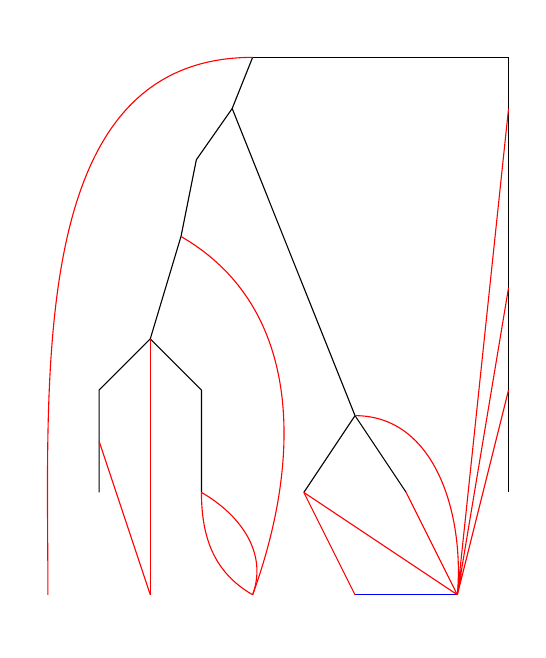
\begin{tikzpicture}[scale=1.3]


\node [] (a) at (0,0.75) {};
\node [] (a) at (1,0.75) {};
\node [] (a) at (2,0.75) {};
\node [] (a) at (2.3,0.8) {};
\node [] (a) at (3,0.75) {};
\node [] (a) at (4,0.75) {};
\node [] (a) at (1.25,0.85) {};


\node [] (a) at (0,1.25) {};
\node [] (a) at (1,1.25) {};
\node [] (a) at (0,1.75) {};
\node [] (a) at (1,1.75) {};
\node [] (a) at (0.5,2.25) {};
\node [] (a) at (0.25,2.27) {};
\node [] (a) at (0.65,2.75) {};
\node [] (a) at (0.8,3.25) {};
\node [] (a) at (0.95,4) {};
\node [] (a) at (1.5,5) {};
\node [] (a) at (1.5,5.2) {};


\draw (0,0.75)--
 (0,1.25) --
(0,1.75)  -- 
(0.5,2.25) -- (0.65,2.75) -- (0.8,3.25)--  (0.95,4) -- (1.3,4.5)--(1.5,5);
\draw (1,0.75) --
(1,1.25) -- (1,1.75)--(0.5,2.25);




\node [] (a) at (2.5,1.5) {};
\node [] (a) at (2.7,1.7) {};
\node [] (a) at (2.3,2) {};

\node [] (a) at (2.1,2.5) {};
\node [] (a) at (1.9,3) {};
\node [] (a) at (1.7,3.5) {};
\node [] (a) at (1.5,4) {};
\node [] (a) at (1.3,4.5) {};
\node [] (a) at (1.6,4.6) {};


\draw (2,0.75)--
(2.5,1.5) --(2.3,2) --
(2.1,2.5)--(1.9,3) -- (1.7,3.5) -- (1.5,4) -- (1.3,4.5);
\draw (3,0.75)--(2.5,1.5);



\node [] (a) at (4,1.25) {};
\node [] (a) at (4,1.75) {};
\node [] (a) at (4,2.25) {};
\node [] (a) at (4,2.75) {};
\node [] (a) at (4,3.25) {};
\node [] (a) at (4,4) {};
\node [] (a) at (4,4.5) {};
\node [] (a) at (4,5) {};

\node [] (a) at (2.75,5) {};


\draw (4,0.75)--
 (4,1.25) --(4,1.75) -- (4,2.25) -- (4,2.75) -- (4,3.25) -- (4,4) -- (4,4.5) -- (4,5)-- (2.75,5)  --  (1.5,5);



\node [blue] (a) at (-0.5,-0.25) {};
\node [blue] (a) at (0.5,-0.25) {};
\node [blue] (a) at (1.5,-0.25) {};
\node [blue] (a) at (2.5,-0.25) {};
\node [blue] (a) at (3.5,-0.25) {};

\node [blue] (a) at (-0.5,-0.5) {};
\node [blue] (a) at (0.5,-0.5) {};
\node [blue] (a) at (1.5,-0.5) {};
\node [blue] (a) at (2.5,-0.5) {};
\node [blue] (a) at (3.5,-0.5) {};


\draw[blue] (2.5,-0.25) -- (3.5,-0.25);

\draw[red] (1.5,-0.25) to [out=150,in=270] (1,0.75);
\draw[red] (1.5,-0.25) to [out=70,in=-30] (1,0.75);
\draw[red] (3.5,-0.25) -- (4,1.75)
 (3.5,-0.25) -- (4,2.75) 
(3.5,-0.25) -- (4,4.5);
\draw[red] (1.5,-0.25) to [out=70,in=-30] (0.8,3.25);

\draw[red] 
(3.5,-0.25) --(2,0.75) 
 (3.5,-0.25) -- (3,0.75) 
 (3.5,-0.25) to [out=85,in=0] (2.5,1.5);  



\draw[red] (2,0.75) -- (2.5,-0.25);


\draw[red] (0.5,-0.25) -- (0,1.25);
\draw[red] (0.5,2.25)-- (0.5,-0.25);

\draw[red] (-0.5,-0.25)  to [out=90,in=180]  (1.5,5);

\end{tikzpicture}
\caption{ is a feedback vertex set of  and the tree  is rooted 
at . Algorithm  will output  and 
 when .} 
\label{fig:atreemarking}
\end{subfigure}
\begin{subfigure}[b]{0.5\textwidth}
        \centering

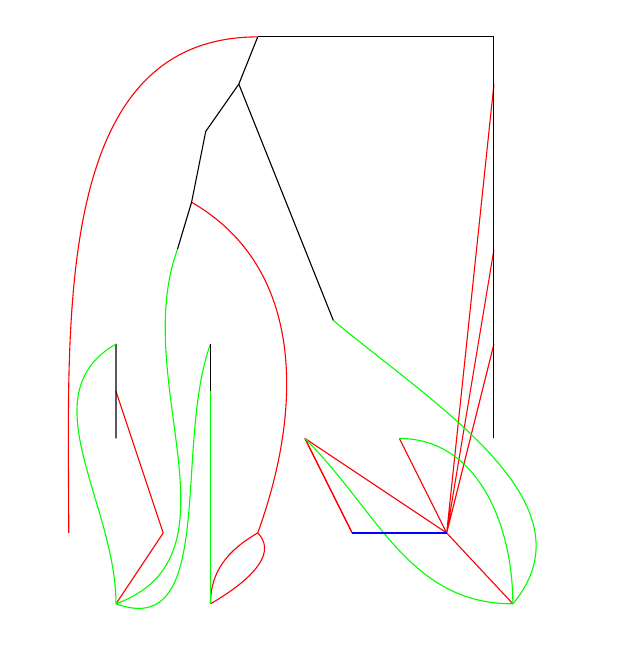
\begin{tikzpicture}[scale=1.2]




\node [] (a) at (-0.25,-1.2) {};
\node [] (a) at (0,-1) {};
\node [] (a) at (1,-1) {};
\node [] (a) at (0.75,-1.2) {};
\node [] (a) at (4.2,-1) {};
\node [] (a) at (4.4,-1.2) {};



\draw[red] (1.5,-0.25) to [out=210,in=90] (1,-1);
\draw[red] (1.5,-0.25) to [out=-45,in=30] (1,-1);

\draw[red] (3.5,-0.25) -- (4,1.75)
 (3.5,-0.25) -- (4,2.75) 
(3.5,-0.25) -- (4,4.5);
\draw[red] (1.5,-0.25) to [out=70,in=-30] (0.8,3.25);

\draw[red] (3.5,-0.25) --(2,0.75) 
 (3.5,-0.25) -- (3,0.75) 
 (3.5,-0.25)--(4.2,-1);


\draw[red] (2,0.75) -- (2.5,-0.25);

\draw[red] (2,0.75) -- (2.5,-0.25);


\draw[red]  (0,-1) -- (0.5,-0.25);
\draw[red] (0,1.25)-- (0.5,-0.25);


\draw[red] (-0.5,-0.25)  to [out=90,in=180]  (1.5,5);



\node [] (a) at (0,0.75) {};
\node [] (a) at (2,0.75) {};
\node [] (a) at (3,0.75) {};
\node [] (a) at (4,0.75) {};
\node [] (a) at (2.75,0.75) {};


\node [] (a) at (0,1.25) {};
\node [] (a) at (1,1.25) {};
\node [] (a) at (0,1.75) {};
\node [] (a) at (1,1.75) {};
\node [] (a) at (0.65,2.75) {};
\node [] (a) at (0.8,3.25) {};
\node [] (a) at (0.95,4) {};
\node [] (a) at (1.5,5) {};

\draw (0,0.75)-- (0,1.25)
 --(0,1.75)
(0.65,2.75) -- 
(0.8,3.25)--  
(0.95,4) -- (1.3,4.5)--(1.5,5);
\draw[green]
(0,1.75) to [out=210,in=90] (0,-1)
(1,1.75) to [out=250,in=-20] (0,-1)
(0.65,2.75) to [out=250,in=20] (0,-1);

\draw [green]
(1,-1)--
(1,1.25);
\draw (1,1.25)
 -- (1,1.75);





\node [] (a) at (2.3,2) {};

\node [] (a) at (2.1,2.5) {};
\node [] (a) at (1.9,3) {};
\node [] (a) at (1.7,3.5) {};
\node [] (a) at (1.5,4) {};
\node [] (a) at (1.3,4.5) {};

\draw[green] (2,0.75) to [out=-45,in=180]
(4.2,-1) to [out=50,in=-40] (2.3,2);
\draw
(2.3,2) --
(2.1,2.5)--(1.9,3) -- (1.7,3.5) -- (1.5,4) -- (1.3,4.5);
\draw[green] (3,0.75)  to [out=0,in=90] (4.2,-1);




\node [] (a) at (4,1.25) {};
\node [] (a) at (4,1.75) {};
\node [] (a) at (4,2.25) {};
\node [] (a) at (4,2.75) {};
\node [] (a) at (4,3.25) {};
\node [] (a) at (4,4) {};
\node [] (a) at (4,4.5) {};
\node [] (a) at (4,5) {};

\node [] (a) at (2.75,5) {};


\draw (4,0.75)--
 (4,1.25) --(4,1.75) -- (4,2.25) -- (4,2.75) -- (4,3.25) -- (4,4) -- (4,4.5) -- (4,5)-- (2.75,5)-- (1.5,5);



\node [blue] (a) at (-0.5,-0.25) {};
\node [blue] (a) at (0.5,-0.25) {};
\node [blue] (a) at (1.5,-0.25) {};
\node [blue] (a) at (2.5,-0.25) {};
\node [blue] (a) at (3.5,-0.25) {};

\node [blue] (a) at (0.25,-0.2) {};
\node [blue] (a) at (1.75,-0.5) {};
\node [blue] (a) at (3.5,-0.5) {};


\draw[blue] (2.5,-0.25) -- (3.5,-0.25);



\end{tikzpicture}
\caption{The vertices of  is drawn separately with edges between  and  colored green}
\label{fig:btreemarking}
\end{subfigure}

\caption{An example of Lemma~\ref{lemma:mark_in_tree}}
\label{fig:treemarking}
\end{figure}
 

\begin{lemma}
\label{lemma:mark_in_tree}
Let  be an instance of \CP{} and let  be a feedback vertex set of . Then there is 
a polynomial time algorithm  that given  and , either outputs  
vertex disjoint cycles in  or two sets  and  such that 
  and  for any  and any connected component  of , 
. 
\end{lemma}
\begin{proof}
We know that  is a forest. We consider each tree in  as a rooted tree, where the root is chosen arbitrarily. Now we create a 
{\em dummy root } and connect to all the roots in . The resulting graph  with vertex set  is 
a tree rooted at . The level of a vertex  is the distance between  and , denoted by . Let  be a rooted tree, then for a vertex   
we use  to denote the subtree of  rooted at .  

Now we are ready to give a procedure to find the desired sets 
 and . Initially we set ,  and . Let  such that 
 is maximized and there is a vertex  with the property that  has a cycle.  
Then, we set ,  and . We continue this procedure until  
or the above step is not applicable. Let .
Notice that by the above process there are vertex disjoint subtrees 
 of   such that for each ,  has a cycle. 
Thus when , our algorithm 
 will output one cycle from each ,  as the output. Otherwise, since in each step the 
algorithm picks a vertex with highest level, each connected component  of  and ,  
. 
Algorithm  will output 
 and  are the required sets. Notice that, in this case . We have seen that there are  vertex disjoint cycles in . This implies that   .  An illustration is given in Figure~\ref{fig:treemarking}.  Figure~\ref{fig:atreemarking} depicts a graph  with a feedback vertex set  and 
the sets  and  chosen by the algorithm. In Figure~\ref{fig:btreemarking}, the graph  is drawn separately 
to see the properties mentioned in the lemma.  
 
\end{proof}

Using Lemma~\ref{lemma:mark_in_tree}, we will prove the following decomposition lemma and after this the structure of the reduced graph becomes ``nice'' and our algorithm boils down to applications of \shortULI{} on multiple auxiliary interval graphs.  


\begin{lemma}
\label{lem:CP_path_creation}
Let  be an instance of \CP. Then there is a polynomial time algorithm  which either 
outputs  vertex disjoint cycles or 
a minor  of , and  with the following properties.
\begin{itemize}
\setlength{\itemsep}{-2pt}
\item[] , 
\item[] , , 
\item[]  is a  collection  of   non trivial paths, and 
\item[] for each path  in , no internal vertex is adjacent to a vertex in , \;
, and .
\end{itemize}
Furthermore, given a cycle packing  in , there is a polynomial time algorithm  which 
outputs a cycle packing  in  such that . 
\end{lemma}

\begin{proof}
We first give a description of the polynomial time algorithm  mentioned in the statement of the lemma. 
It starts by running  the algorithm mentioned in Lemma~\ref{lemma:erdosposa} on input  and if it returns  vertex disjoint cycles,  then  returns 
 vertex disjoint cycles in  
and stops. Otherwise, let  be a 
feedback vertex set of . 
Now   applies Reduction Rule~\ref{rule:leaf} repeatedly using the feedback vertex set  until 
Reduction Rule~\ref{rule:leaf} is no longer applicable. Let  be the reduced instance after the exhaustive application of 
Reduction Rule~\ref{rule:leaf}. By Lemma~\ref{lemma:leaf}, we have that  and  is a forest. 
Now,   runs the algorithm  mentioned in Lemma~\ref{lemma:mark_in_tree} on input  and . If  
returns  vertex disjoint cycles in , then  also returns  vertex disjoint cycles in . The last assertion follows from the fact that  Reduction Rule~\ref{rule:leaf} (applied to get ) is \onesafe. 
Otherwise, let  and  be the output of . Next we define a 
few sets that will be used by  to construct its output.
\begin{enumerate}
\setlength{\itemsep}{-2pt}
\item Let  be the set 
of vertices of  whose  degree in  is at least . 
\item Let ; and 
\item let  be the vertices of degree  in . 
\end{enumerate}
Algorithm  returns ,  and 
 as output. In the example given in Figure~\ref{fig:treemarking},  and .

Now we prove the correctness of the algorithm. If  outputs  vertex disjoint  cycles in , then we are done. Otherwise, let  and  be the output of . 
Now we prove  and   indeed satisfy the properties mentioned in the statement of lemma.
Since  is obtained after repeated applications of Reduction Rule~\ref{rule:leaf}, by Observation~\ref{obs:leaf_opt}, we get 
that  and hence proving property .  


By Lemma~\ref{lemma:mark_in_tree}, 
we have that . Hence the size of  is as desired. 
Next we bound the size of .  
By  Lemma~\ref{lemma:erdosposa}, we have that , where  is a fixed constant.   
By Lemma~\ref{lemma:leaf}, we have that ,  is a forest, and 
the number of vertices of  degree at most  in  is upper bounded by . 
Since the number of vertices of degree at least  in a forest is at most the number of leaves in the forest, we can conclude 
that cardinality of , the set of vertices of degree at least  in  is upper bounded by . It is well-known that the number of maximal degree  paths in a forest is  upper bounded by the sum of the number of leaves and the vertices of degree at least  
(for example see~\cite{RamanSS06} for a proof). This immediately implies the following claim. 

\begin{claim}
 \label{claim:no_of_paths}
  is a collection of  paths. 
\end{claim}
The following claim proves properties  and  stated in the lemma. 
\begin{claim}
\label{claim:CPboundR}
 and the number of paths in  is at most  . 
\end{claim}
\begin{proof}
Observe that  is a 
collection of  paths and thus it has at most   connected components. This implies that,  has at most   connected components and in particular  has at most   connected components. 
Let  denote the number of connected components of . 
By Lemma~\ref{lemma:mark_in_tree}, we have that 
for any  and any connected component  of , 
.  Thus, for every vertex   we have that 
. 
This
implies that the cardinality of , the set ,  
is upper bounded by .  
By Lemma~\ref{lemma:mark_in_tree}, we have that . 
Since  and by Claim~\ref{claim:no_of_paths}, we can conclude 
that the number of paths in  is at most . 
Notice that  is the family of paths on single vertices in the collection of paths of 
. 
Since the number of maximal paths in  is at most , 
we have that  and 
the number of maximal paths in  (i.e, the 
number of paths in ) is at most . 

Since , , ,  and , we can conclude that the cardinality of 
, is upper bounded by . This concludes the proof. 
\end{proof}
Finally, we will show the last property stated in the lemma. 
Since  is a forest and  is the set of vertices of degree at least  in the forest , 
we have that  any internal vertex of any path in  is not adjacent to . 
Also, since any vertex , which is an internal vertex of a path in  and 
adjacent to a vertex in , belongs to , we can conclude that no internal vertex of any path in  is adjacent to 
. This implies that  
no internal vertex of any path in  is adjacent to 
.  
Now we claim that an endpoint  of a path  in  has at most 
one edge between  and . 
Let  be an endpoint of . 
Since   and , we can conclude that  is not adjacent to 
any vertex in . 
Since , the degree of 
 in  is at most . Since  is a non trivial path . 
Since  is a forest, , and  is not adjacent to any vertex in , 
we conclude that .  

The solution lifting algorithm, ,  is basically obtained by solution lifting algorithm 
used in the Reduction Rule~\ref{rule:leaf}. That is,   given a cycle packing  in ,   
repeatedly applies the solution lifting algorithm of  Reduction Rule~\ref{rule:leaf} to obtain a cycle packing  in  such that . The correctness of the algorithm  follows 
from the fact that Reduction Rule~\ref{rule:leaf} is \onesafe, 
and  is obtained from  by repeated application of 
Reduction Rule~\ref{rule:leaf}.  
An illustration of a path ,  and  can be found in Figure~\ref{figure_CP_paths}. 
This completes the proof of the lemma. 
\end{proof}


 
 \begin{figure}

\centering

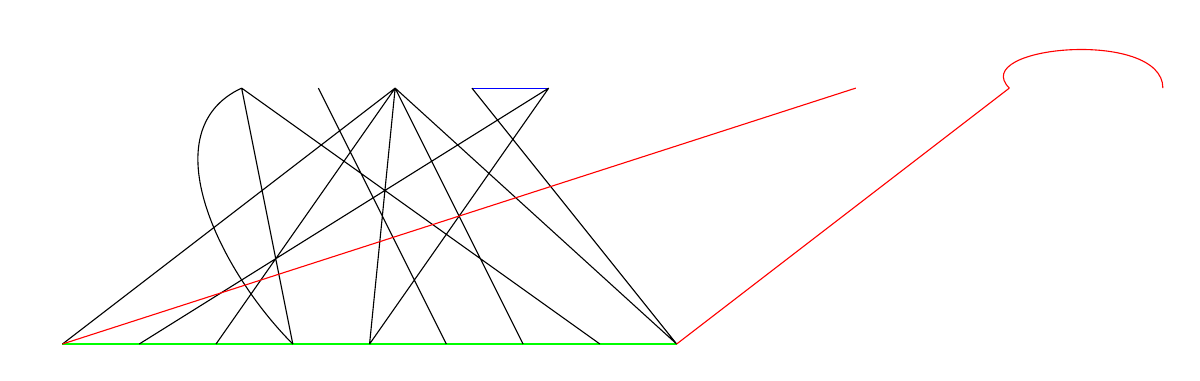
\begin{tikzpicture}[rotate=90, scale=1.3]


\node [green] (a) at (0.2,7) {};
\node [green] (a) at (0,0.75) {};
\node [green] (a) at (0,1.5) {};
\node [green] (a) at (0,2.25) {};
\node [green] (a) at (0,3) {};
\node [green] (a) at (0,3.75) {};
\node [green] (a) at (0,4.5) {};
\node [green] (a) at (0,5.25) {};
\node [green] (a) at (0,6) {};
\node [green] (a) at (0,6.75) {};



\node [blue] (a) at (2.6,6) {};
\node [blue] (a1) at (2.5,2) {};
\node [blue] (a2) at (2.5,2.75) {};
\node [blue] (a) at (2.5,3.5) {};
\node [blue] (a) at (2.5,4.25) {};
\node [blue] (a) at (2.5,5) {};


\node [] (a) at (2.8,2) {};
\node [] (a) at (2.8,2.75) {};
\node [] (a) at (2.8,3.5) {};
\node [] (a) at (2.8,4.25) {};
\node [] (a) at (2.8,5) {};

\draw[blue] (2.5,2)--(2.5,2.75);


 \draw[green] (0,0.75)-- (0,1.5) --(0,2.25) --
(0,3) --
 (0,3.75)-- 
 (0,4.5)-- 
 (0,5.25)--(0,6) --(0,6.75); 

 \draw[black]
(0,0.75)--(2.5,2.75)
(0,0.75)--(2.5,3.5) 
(0,1.5) --(2.5,5)
(0,2.25) --(2.5,3.5)
(0,3) --(2.5,4.25)
 (0,3.75)-- (2.5,2)
 (0,4.5)-- (2.5,5)
 (0,5.25)--(2.5,3.5)
(0,6) --(2.5,2)
(0,6.75)-- (2.5,3.5)
(0,3.75)--(2.5,3.5)
; 

\draw(0,4.5) to[out=45,in=115] (2.5,5);

\node [red] (a) at (2.5,-4) {};
\node [red] (a) at (2.5,-3.25) {};
\node [red] (a) at (2.5,-2.5) {};
\node [red] (a) at (2.5,-1.75) {};
\node [red] (a) at (2.5,-1) {};
\node [red] (a) at (2.5,0) {};

\draw[red] (2.5,-2.5)--(0,0.75);
\draw[red] (2.5,-1)--(0,6.75);

\draw[red] (2.5,-4) to[out=0,in=45] (2.5,-2.5);


\end{tikzpicture}

\caption{An example of a path  in ,  and }
\label{figure_CP_paths}
\end{figure}


 
Observe that Lemma~\ref{lem:CP_path_creation} decomposes the graph into  simple structures, namely, paths in   combined together with a set of size . Note that the only {\em unbounded} objects in  are the paths in . The reason we can not reduce the size of  is that a vertex in  can have unbounded neighbors on it. See Figure~\ref{figure_CP_paths} for an illustration. However,  
Lemma~\ref{lem:CP_path_creation} still  provides us the required decomposition which will be used to cast several instances of 
\shortULI{}. In particular for every path , we will have one instance of 
\shortULI{}. We will compute \shortuli{} for each of these instances and reduce the path size to get the desired kernel. 





\begin{theorem}
\label{thm:CPapprx}
For any , there is polynomial sized -approximate kernel for \CP. That is, \CP{} admits a PSAKS. 
\end{theorem}
\begin{proof}
Let  be an input instance of \CP.  
The reduction algorithm  works as follows. It first runs the algorithm  mentioned in Lemma~\ref{lem:CP_path_creation}. If the algorithm returns  vertex disjoint cycles, then  return these cycles. Otherwise, let ,  and  be the output of , satisfying four properties mentioned in Lemma~\ref{lem:CP_path_creation}. Important properties that will be most useful in our context are: 


\begin{itemize}
\setlength{\itemsep}{-2pt}
\item , ; and 
\item   is a collection  of non trivial  
paths such that for any path  we have that no internal vertex of  is adjacent to  
any vertex of .
\end{itemize}
\noindent 
Now  will solve several instances of  \shortULI{} to bound the length of each path in 
. Towards this we fix a path  
Our objective is to apply Lemma~\ref{lem:uni_lab_is} 
to reduce the length of . 
Our algorithm finds a set of small number of relevant vertices on  
and reduces  in {\em a single step} even though 
we use Lemma~\ref{lem:uni_lab_is} several times to identify relevant vertices.  Next we give the  construction for applying Lemma~\ref{lem:uni_lab_is} in order to find the relevant vertices. To find relevant vertices of , we create  labelled interval graphs, one for every 
  
with  being the set of labels. That is, for  the path  and  we create a  labelled interval graph  as follows. Our labelling function will be denoted by  .

\begin{enumerate}
\setlength{\itemsep}{-2pt}
\item The set of labels is . 
\item Let  be the subpath of  such that  is the first vertex in  adjacent to  and  is the last vertex on  adjacent to .  If , then  and if , then . Indeed, if  and  then  and . 
\item We say that a subpath  of  is a {\em potential -subpath}, 
where , if   
either  or  is an induced path (induced cycle when ) in . Essentially, the potential subpath is trying to capture the way a cycle can interact with a subpath in  with its neighbors on the cycle being  and .
\item For each  
and a potential -subpath  we create an interval  
 and  label it with . That is, . 
We would {\em like to emphasize} that when  and , we create an interval  only if 
there are two edges between  and .  
Also notice that if we have created an interval  with label , then we have created an interval  with label  as well.  
\end{enumerate}

\begin{figure}

\centering

\begin{tikzpicture}[ scale=1.3]


\node [] (a) at (0.4,0) {};
\node [] (a) at (0.75,0) {};
\node [] (a) at (1.5,0) {};
\node [] (a) at (2.25,0) {};
\node [] (a) at (3,0) {};
\node [] (a) at (3.75,0) {};
\node [] (a) at (4.5,0) {};
\node [] (a) at (5.25,0) {};
\node [] (a) at (6,0) {};
\node [] (a) at (6.75,0) {};
\node [] (a) at (7.5,0) {};



\node [blue] (a) at (1.5,1.5) {};
\node [blue] (a1) at (2,1.5) {};
\node [blue] (a2) at (2.75,1.5) {};
\node [blue] (a) at (3.5,1.5) {};
\node [blue] (a) at (4.25,1.5) {};
\node [blue] (a) at (5,1.5) {};


\node [] (a) at (2,1.8) {};
\node [] (a) at (2.75,1.8) {};
\node [] (a) at (3.5,1.8) {};
\node [] (a) at (4.25,1.8) {};
\node [] (a) at (5,1.8) {};




 \draw[] (0.75,0)-- (1.5,0) --(2.25,0) --
(3,0) --
 (3.75,0)-- 
 (4.5,0)-- 
 (5.25,0)--(6,0) --(6.75,0)--(7.5,0); 

 \draw[black]
(2,1.5) -- (1.5,0)
(5,1.5)-- (6,0)
(2,1.5) -- (2.25,0)
(2,1.5) -- (4.5,0)
(2.75,1.5)-- (3.75,0)
(2.75,1.5)-- (5.25,0)
(4.25,1.5)to[out=-10,in=60](5.25,0)
(4.25,1.5)to[out=-90,in=100](5.25,0)
(3.5,1.5)--(0.75,0)
; 



\node [] (a) at (3,-0.4) {};
\draw[line width=0.35mm,red] (2.25,-0.53)--(3.75,-0.53); 
\node [] (a) at (4.9,-0.4) {};
\draw[line width=0.35mm,red] (2.25,-0.65)--(3.75,-0.65);
\node [] (a) at (3,-0.8) {};
\node [] (a) at (4.9,-0.8) {};
\draw[line width=0.35mm,red] (4.5,-0.53)-- (5.25,-0.53);
\draw[line width=0.35mm,red] (4.5,-0.65)-- (5.25,-0.65);
\node [] (a) at (5.8,-1.4) {};
\node [red] (a) at (5.25,-1.4) {};


\draw[line width=0.35mm,red] (2.25,-1.2)--(4.5,-1.2);
\node [] (a) at (3.5,-1.05) {};

\node [] (a) at (4.2,-1.45) {};
\draw[line width=0.35mm,red] (3.75,-1.6)--(4.5,-1.6);
\draw[line width=0.35mm,red] (3.75,-1.75)--(4.5,-1.75);
\node [] (a) at (4.2,-1.85) {};

\draw[thick, dotted] (0,-2)--(8,-2);
\node [] (a) at (.75,-2.15) {};
\node [] (a) at (1.5,-2.15) {};
\node [] (a) at (2.25,-2.15) {};
\node [] (a) at (3,-2.15) {};
\node [] (a) at (3.75,-2.15) {};
\node [] (a) at (4.5,-2.15) {};
\node [] (a) at (5.25,-2.15) {};
\node [] (a) at (6,-2.15) {};

\end{tikzpicture}

\caption{An example of .  The interval representation of  along with labels is drawn below 
the path . The real line is represented using a dotted line.}
\label{figure_HP}
\end{figure}



This completes the construction of     and the labelling function
 .  
See Figure~\ref{figure_HP} for an illustration.  
The fact that   is an interval graph follows from the fact that in fact to construct  , we have given an interval representation for it. 
Having, created the interval graph and a labelling function  runs the following steps. 



\begin{enumerate}
\setlength{\itemsep}{-2pt}
\item Now using Lemma~\ref{lem:CP_path_creation},   computes 
a set  such that  is a \shortuli{} of . 
Now we define a few sets. 




\item Now,  will do the following modification to  shorten : delete all the edges between 
 and , and then contract all the remaining edges incident with vertices in . In other words, let , where . Then delete  and add edges . 
Let  be the path obtained from , by the above process. We use the same vertex names in  as well to represent a
vertex. That is, if a vertex  in  is not deleted to obtain , we use  to represent the same vertex. 
\item Let  be the graph obtained after this modification has been done for all paths . 
Finally,   returns  as the reduced instance. 
\end{enumerate}
\paragraph{Solution Lifting Algorithm.} 
Notice that  is a minor of  and hence a minor of .  Given a set  of vertex disjoint cycles in 
, the solution lifting algorithm computes a set  of vertex disjoint cycles in  of cardinality 
 by doing reverse of the minor operations used to obtain  from . All this can be done in polynomial time because  the solution lifting algorithm knows the 
minor operations done to get  from .    

Next we need to prove the correctness of the algorithm. Towards that we first bound the size of .  

\medskip
\noindent 
{\bf Bounding the size of .} As a first step to bound the size of , we bound the chromatic number of , where  and 
. In fact what we will bound is the size of the maximum clique of . 
\begin{claim}
\label{claim:CPpw}
For any  and , . 
\end{claim}
\begin{proof}
To prove the claim, it is enough to show that the size of a maximum clique in  is at most . 
Let . We know that in the interval representation of ,  
all the intervals are contained in . We claim that for any point  and ,  
the number of intervals labelled  and containing the point  is at most . Towards a contradiction assume that there are 
three intervals  such that  and all the 
intervals ,  and  contain the point . Since for each  and  
we have created at most one interval  with label , all the intervals  and  are distinct intervals in the real line. 

We first claim that no interval in  is same as . Suppose . 
Since all the interval in , are different and  we have that 
, but contains . This implies that either  or . We consider 
the case . The case that   is symmetric. 
Let . 
We know that  is an induced 
path (induced cycle when  and two edges between  and ). This 
implies that neither  nor  is an induced path, 
because . We would like to clarify that  
when  and ,  is cycle 
and there are two edges between  and . 
This implies that  is a not an induced cycle.
 See Figure~\ref{figure_pointinterval} for illustration.  



\begin{figure}
\begin{subfigure}[b]{0.5\textwidth}
        \centering

\begin{tikzpicture}[ scale=1]

\node[blue] at (-0.8,1.5) {};
\node [blue] (a) at (-0.5,1.5) {};
\node [blue] (a) at (2.5,1.5) {};
\node[blue] at (2.8,1.5) {};

\draw[line width=0.35mm,red] (0,0)--(2,0);
\node [red] (a) at (0,0) {};
\node [red] (a) at (2,0) {};
\node [red] (a) at (1,0.8) {};
\node [red] (a) at (1,0.5) {};
\node [red] (a) at (1,-0.3) {};
\node [red] (a) at (1,0) {};

\draw[thick, dotted] (-0.5,1.5) -- (0,0);
\draw[thick, dotted] (-0.5,1.5) -- (1,0);
\draw[thick, dotted] (2.5,1.5) -- (2,0);
\draw[thick, dotted] (2.5,1.5) -- (1,0);




\node[blue] at (4.2,1.5) {};
\node [blue] (a) at (4.5,1.5) {};


\draw[line width=0.35mm,red] (5,0)--(7,0);
\node [red] (a) at (5,0) {};
\node [red] (a) at (7,0) {};
\node [red] (a) at (7,0.8) {};
\node [red] (a) at (7,0.5) {};
\node [red] (a) at (6,-0.3) {};
\draw[thick, dotted] (4.5,1.5) -- (5,0);
\draw[thick, dotted] (4.5,1.5) -- (7,0);
\draw[thick, dotted] (4.5,1.5)  to[out=0,in=120] (7,0);
\end{tikzpicture}
\end{subfigure}
\begin{subfigure}[b]{0.5\textwidth}
        \centering

\begin{tikzpicture}[ scale=1]

\node[blue] at (-0.8,1.5) {};
\node [blue] (a) at (-0.5,1.5) {};
\node [blue] (a) at (2.5,1.5) {};
\node[blue] at (2.8,1.5) {};

\draw[line width=0.35mm,red] (0,0)--(2,0);
\draw[line width=0.35mm,red] (1,0.7)--(1.8,0.7);
\draw[line width=0.35mm,red,dotted] (1.8,0.7)--(3,0.7);
\node [red] (a) at (0,0) {};
\node [red] (a) at (2,0) {};
\node [red] (a) at (1,0.5) {};
\node [red] (a) at (1,-0.3) {};
\node [red] (a) at (1,0) {};

\draw[thick, dotted] (-0.5,1.5) -- (0,0);
\draw[thick, dotted] (-0.5,1.5) -- (1,0);
\draw[thick, dotted] (2.5,1.5) -- (2,0);



\end{tikzpicture}
\end{subfigure}
\caption{Illustration of 
proof of Claim~\ref{claim:CPpw}. The case when  is drawn in the left and middle figures. 
The figure in the middle represents the 
case when  and .
The case when  and  intersects at strictly more than one point can be seen in the  right most figure.  
The black dotted curves represent the edges in the graph. }
\label{figure_pointinterval}
\end{figure}







Since  is a common point in ,  and  and none of these intervals is equal to , there are two intervals in 
 such that they intersect at strictly more than one point. 
Without loss of generality we assume that the intersection of   and 
contains at least  points. Also, since  and  are different intervals 
on the real line, one endpoint of an interval is fully inside another interval (not as the endpoint of the other interval). Let . 
Assume that . All other cases are symmetric to this case.  
We know that   or .
This implies that 
neither  nor  is an induced path. This contradicts the fact that we created an interval 
 with label . See Figure~\ref{figure_pointinterval} for illustration.  


We have proved that for any point , the number of intervals containing    with the same label is upper bounded by  . This implies that the cardinality of a largest clique in  is at most twice the number of labels. Thus, the size of the largest cliques is upper bounded by . 
By  Lemma~\ref{lem:CP_path_creation}, we know that  and thus 
 is bounded by . Since the chromatic number of an interval graph is upper bounded by the size of a maximum clique, the proof of the claim follows.  
\end{proof}




By 
Lemma~\ref{lem:CP_path_creation}, we know that 
. 
For each  and , we created a subset 
 of  of cardinality . Hence, the cardinality of  is also upper bounded by . 
The cardinality of   is 
at most . 
This implies that the reduced path  has at most  vertices. 
Also, we know that , hence the total number of vertices across all the paths of  after the reduction is upper bounded by . 
This together with the fact that  and   imply that   is upper bounded by . This completes the proof of upper bound on the size of . 


\medskip
\noindent 
{\bf Correctness of lossy reduction.} Finally, we show that indeed  is a  
-approximate kernel for \CP. Towards this we show the following claim. 

\begin{claim}
\label{claim:optCP}
. 
\end{claim}
\begin{proof}
Let  be an optimum solution to . Without loss of generality we can assume that 
each cycle in  is a {\em chordless cycle}.  
Let  be the non-empty subpaths of cycles in  induced in the graph . 
That is,  is the collection of supaths in the intersection of  and .
For any , 
there exists two vertices  such that  is a subpath in .
Because of property  of Lemma~\ref{lem:CP_path_creation}, for any  with , at least one of the endpoint of  is connected to a vertex from  in the cycle packing . 
We say a path  is a {\em substitute} for  if  is a subpath in  where 
 and  is a subpath in . 
In what follows,   for at least  paths in , we identify substitutes in 
the reduced graph  which are pairwise vertex disjoint.




We partition the paths in  into  and . 
Notice that  is a subpath of a cycle  and the neighbors (could be the same) 
of  both the endpoints  of  on  are in 
. If the neighbors of both endpoints of   on  are in , then we include  in .  Otherwise  is in . 
See Figure~\ref{figure_cyclepathintersection} for an illustration. 
For each , we give a substitute path 
as follows. 
We know that there is a path  such that  either  or  for some  where  can be 
an empty set too.
If , then we replace  with  
(Note that  is the path obtained from  in the reduction process). Also, notice that end vertices of  and  are same 
(because endvertices of  belong to ) 
and hence  is a substitute for 
. Suppose  where . Let  be the cycle in  such that  is a subpath of . 
Let . Let  be the neighbour of  in  which is from  (recall that 
 no internal vertex of  is adjacent to  any vertex of ).  
Since 
 is a chordless cycle, none of  is adjacent to . This implies that   and hence 
 contains a subpath  from  to  with internal vertices from . In this case 
 is a substitute for . In a similar way, we can construct a substitute for  when   where . 
Let  be the set of substitute paths constructed for paths in . Notice that  
is a collection of vertex disjoint paths in  and it has one substitute path for each . 
See Figure~\ref{figure_cyclepathintersection} for an illustration. 




\begin{figure}

\begin{subfigure}[b]{0.5\textwidth}
        \centering
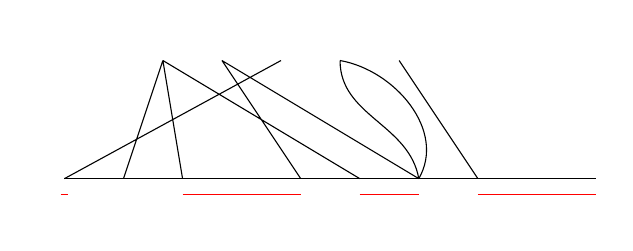
\begin{tikzpicture}[ scale=1]


\node [] (a) at (0.4,0) {};
\node [] (a) at (0.75,0) {};
\node [] (a) at (1.5,0) {};
\node [] (a) at (2.25,0) {};
\node [] (a) at (3,0) {};
\node [] (a) at (3.75,0) {};
\node [] (a) at (4.5,0) {};
\node [] (a) at (5.25,0) {};
\node [] (a) at (6,0) {};
\node [] (a) at (6.75,0) {};
\node [] (a) at (7.5,0) {};

\node [blue] (a) at (1.5,1.5) {};
\node [blue] (a1) at (2,1.5) {};
\node [blue] (a2) at (2.75,1.5) {};
\node [blue] (a) at (3.5,1.5) {};
\node [blue] (a) at (4.25,1.5) {};
\node [blue] (a) at (5,1.5) {};


\node [] (a) at (2,1.8) {};
\node [] (a) at (2.75,1.8) {};
\node [] (a) at (3.5,1.8) {};
\node [] (a) at (4.25,1.8) {};
\node [] (a) at (5,1.8) {};



 \draw[] (0.75,0)-- (1.5,0) --(2.25,0) --
(3,0) --
 (3.75,0)-- 
 (4.5,0)-- 
 (5.25,0)--(6,0) --(6.75,0)--(7.5,0); 

 \draw[black]
(2,1.5) -- (1.5,0)
(5,1.5)-- (6,0)
(2,1.5) -- (2.25,0)
(2,1.5) -- (4.5,0)
(2.75,1.5)-- (3.75,0)
(2.75,1.5)-- (5.25,0)
(4.25,1.5)to[out=-10,in=60](5.25,0)
(4.25,1.5)to[out=-90,in=100](5.25,0)
(3.5,1.5)--(0.75,0)
; 


 \draw[red] (0.7,-0.2)-- (0.8,-0.2) 
(2.25,-0.2) --(3.75,-0.2) 
 (4.5,-0.2)--(5.25,-0.2)
(6,-0.2) --(6.75,-0.2)--(7.5,-0.2); 

\node [] (a) at (0.78,-0.45) {};
\node [] (a) at (3,-0.45) {};
\node [] (a) at (5,-0.45) {};
\node [] (a) at (6.5,-0.45) {};
\end{tikzpicture}
\end{subfigure}
\begin{subfigure}[b]{0.5\textwidth}
        \centering
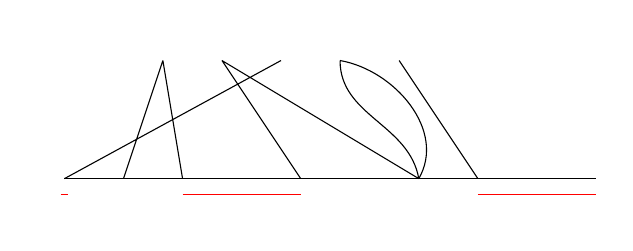
\begin{tikzpicture}[ scale=1]


\node [] (a) at (0.4,0) {};
\node [] (a) at (0.75,0) {};
\node [] (a) at (1.5,0) {};
\node [] (a) at (2.25,0) {};
\node [] (a) at (3.75,0) {};
\node [] (a) at (5.25,0) {};
\node [] (a) at (6,0) {};
\node [] (a) at (7.5,0) {};

\node [blue] (a) at (1.5,1.5) {};
\node [blue] (a1) at (2,1.5) {};
\node [blue] (a2) at (2.75,1.5) {};
\node [blue] (a) at (3.5,1.5) {};
\node [blue] (a) at (4.25,1.5) {};
\node [blue] (a) at (5,1.5) {};


\node [] (a) at (2,1.8) {};
\node [] (a) at (2.75,1.8) {};
\node [] (a) at (3.5,1.8) {};
\node [] (a) at (4.25,1.8) {};
\node [] (a) at (5,1.8) {};



 \draw[] (0.75,0)-- (1.5,0) --(2.25,0) --
(3,0) --
 (3.75,0)-- 
 (4.5,0)-- 
 (5.25,0)--(6,0) --(6.75,0)--(7.5,0); 

 \draw[black]
(2,1.5) -- (1.5,0)
(5,1.5)-- (6,0)
(2,1.5) -- (2.25,0)
(2.75,1.5)-- (3.75,0)
(2.75,1.5)-- (5.25,0)
(4.25,1.5)to[out=-10,in=60](5.25,0)
(4.25,1.5)to[out=-90,in=100](5.25,0)
(3.5,1.5)--(0.75,0)
; 


 \draw[red] (0.7,-0.2)-- (0.8,-0.2) 
(2.25,-0.2) --(3.75,-0.2) 
(6,-0.2) --(6.75,-0.2)--(7.5,-0.2); 

\node [] (a) at (0.78,-0.45) {};
\node [] (a) at (3,-0.45) {};
\node [] (a) at (6.5,-0.45) {};
\end{tikzpicture}
\end{subfigure}




\caption{An example of intersection of  and a path . 
The vertices in  colored black belong to . 
The intersection of  and  are the set of paths 
. Here  and . 
The substitute paths for  is in the figure at the right hand side}
\label{figure_cyclepathintersection}
\end{figure}


































Now we construct substitute paths for . Here, we construct substitute paths for at least  
paths and these paths will be vertex disjoint. Moreover, these paths will be vertex disjoint from the paths in  as well. 
Let  be a path in  such that at least one path in  is a subpath of . 
Let  be a subset of  containing all the paths in  that is a subpath of . 
There are at most two paths in  which 
are subpaths of . Let  and  be these paths, where  and  could be empty too. 
 Let the neighbours of  and  in  in the cycle packing  be  and , respectively 
(here,  if  and  if ).  
Then, consider the  following decomposition of path . We claim that . That is,  is a path for which we would have created the interval graph .  
Observe that, if  is non-empty then   does not have any neighbor on  as cycles in  are {\em chordless}. Similarly, if  is non-empty then  does not have any neighbor on . 
Thus, if  and  are both non-empty then indeed the {\em last} vertex of  is the {\em first}  vertex on  that is a neighbor of  and the {\em first} vertex of  is the {\em last} vertex on  that is a neighbor of . This implies that indeed we would have created the interval graph . We can argue similarly if either  is empty or  is empty.  
Now consider the interval graph . This graph is constructed from . 
Since 
each cycle in  is a chordless cycle, we have that 
each subpath  is a potential -subpath of  where 
either  or  is a subpath of  and .
Since each vertex in  has degree two in , 
for a pair  we have {\em at most two potential  paths} 
 and  in . Also note that these supaths  and  are 
potential -subpaths as well. So when there are two paths  
such that  and  are subpaths of , then we consider  
as a potential -subpath and  as  a potential -subpath.  
Now we can consider  as a set of potential subpaths of . 
That is, for each 
, there is an interval  with label  
and  is not a label of any other intervals corresponding to a subpath in 
.
Let  be the set of interval created for the potential subpaths in . 
We have explained that for 
any , there is at most one potential -subpath in . 
Also notice that, since  is a collection of vertex disjoint paths, the interval 
constructed for corresponding potential subpaths are disjoint. This 
implies that  is an independent set in   and 
. 
By Lemma~\ref{lem:uni_lab_is}, we have that 
there is a subset 
such that there is an independent set  of cardinality 
in  and . This implies that there are at least 
 
of paths in  has {\em substitute paths} in  which are vertex disjoint from 
 and , where  is the path obtained from  in the reduction process using Lemma~\ref{lem:uni_lab_is}. This implies that for 
each , at least  paths has 
substitute paths in  and they are vertex disjoint subpaths of  and does not intersect 
with  and . We denote the set of substitute paths in  by . 
This implies that the substitute paths for  are vertex disjoint and they are vertex disjoint from the 
substitute paths for . Let these substitute paths form a set . 
Also notice that 
since each vertex , has degree at most  in  and , 
the total number of paths in  is at most .
From each , at least  paths have 
substitute paths in . Recall that, 

That is,  () is the disjoint union of  () for . Thus, 

This implies that . This implies that   contains at least  substitute paths. Each path in  for which we do not have a substitute path can destroy at most one cycle in 
. Recall that,   is an optimum solution to . This implies that 
contains at least  vertex disjoin cycles. 
This completes the proof of the claim. 
\end{proof}
By Lemma~\ref{lem:CP_path_creation}, we know that  and hence 
by Claim~\ref{claim:optCP} we get that .   
We know that given a solution  of  the solution lifting algorithm will output a solution  of same cardinality
for . Therefore, we have  

This gives the desired PSAKS for \CP{} and completes the proof.
\end{proof}


